\documentclass[12pt]{article}
\usepackage{amsmath}
\usepackage{mathtools}
\usepackage{bigints}
\usepackage{parskip}
\usepackage{amssymb}
\usepackage{relsize}
\usepackage{fullpage}

\usepackage{hyperref}



	\addtolength{\topmargin}{-.875in}
	\addtolength{\textheight}{1.75in}



    \newenvironment{myindentpar}[1]%
     {\begin{list}{}%
             {\setlength{\leftmargin}{#1}}%
             \item[]%
     }
     {\end{list}}

\begin{document}
\title{Math for Business Study Guide Midterm 1}
\date{Fall 2014}
\maketitle

\textbf{NOTE:} This is intended as a study aid for the first midterm. This is not an official study guide. It is just something that I create on my own in the hopes that you find it useful. The supervising professor for the course has nothing to do with the creation of this study guide. There are likely things that will be covered in the midterm that I don't put on here so it's ultimately up to you as the student to make sure you're properly prepared. However, that being said, I do try to cover the main topics and it's helpful to have one document to look at that lists most of the formulas you need to know for the midterm. I do try to cover all of the main topics, but for brevity, I often leave out certain things that I see as a being easier which you could just as easily learn from the textbook/internet/elsewhere. 



\section{Chapter 1: Functions and Their Graphs}

\subsection{Functions}

\textbf{Domain} - the set of numbers that you can input into your function

\begin{myindentpar}{1cm}
\textbf{Note:} Usually you need to be careful of two types of functions: 

\begin{enumerate}
\item \textbf{square root function} 

The function $f(x) = \sqrt{x}$ has a domain $x \geq 0$. 

You may also see something like $f(x) = \sqrt{(x-1)(5-x)(x+7)}$ and be asked to find the domain. 

You then need to solve $(x-1)(5-x)(x+7) \geq 0$ to find the domain

\textbf{Note:} This also holds for fourth roots: $\mathlarger{\mathlarger{\mathlarger{\sqrt[4]{x}}}}$, $\mathlarger{\mathlarger{\mathlarger{\sqrt[6]{x}}}}$ or any even root. The domain of odd roots such as $\mathlarger{\mathlarger{\mathlarger{\sqrt[3]{x}}}}$, $\mathlarger{\mathlarger{\mathlarger{\sqrt[5]{x}}}}$ etc... is all reals
\item \textbf{rational function}

 A rational function is of the form $f(x) = \dfrac{P(x)}{R(x)}$ where $P(x)$ and $R(x)$ are polynomial. The domain of a rational function is all reals except for $R(x)=0.$ 

For example the domain of $f(x) = \dfrac{x^2+3x+1}{x-1}$ is $(-\infty, 1) \cup (1, \infty)$
\end{enumerate}

 Sometimes you might see a combination of both. 

For example, find the domain of $f(x) = \dfrac{1}{\sqrt{(3-x)(2+x)}}$ 

We do this by solving $(3-x)(2+x)>0$
\end{myindentpar}

Graphically, you can determine the domain by scanning along the x-axis and seeing what x-values the function is not defined for.

\textbf{Range} - the set of numbers that are output from a function. Often harder to determine than the domain, we can determine the range graphically by scanning along the y-axis and seeing what y-values the function is not defined for.

\vspace{2cm}

\textbf{Internet Links:}

\begin{itemize}
\item \href{https://www.youtube.com/watch?v=hZEGZMb4uzQ}{mathbff - Domain} 

\item \href{https://www.khanacademy.org/math/algebra/algebra-functions/domain_and_range/v/domain-and-range-1}{Khan Academy - Domain and Range}

\end{itemize}


\textbf{Vertical Line Test:} - a nice, easy, graphical test to determine if a graph is a function. It says that a graph of an equation is a function is any vertical line that can be drawn intersects the graph in \textbf{no more than one point}.

\begin{myindentpar}{1cm}

\textbf{Graph That Passes the Vertical Line Test:}

\centerline{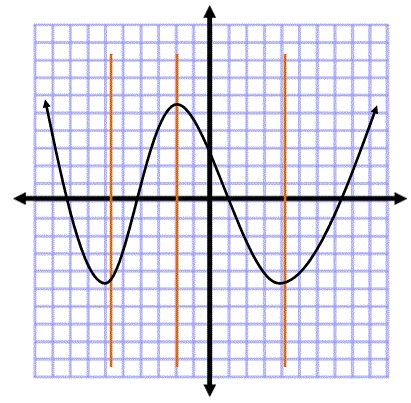
\includegraphics{PassesVLT.jpg}}

\newpage

\textbf{Graph That Fails the Vertical Line Test:}

\centerline{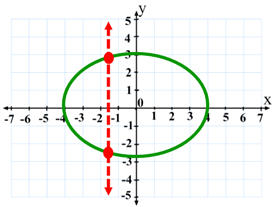
\includegraphics{FailsVLT.jpg}}

\end{myindentpar}

\subsection{Graphs of Functions}


{\bf \underline{Even \& Odd Functions}}
\begin{myindentpar}{1cm}
\textbf{Even Function} - a function is \textit{even} if $f(-x) = f(x)$ Even functions always have y-axis symmetry

\textbf{Odd Function} - a function is \textit{odd} if $f(-x) = -f(x)$ Odd functions always have origin symmetry
\end{myindentpar}

\textbf{Graph of Quadratic Function $\mathbf{y=x^2}$}

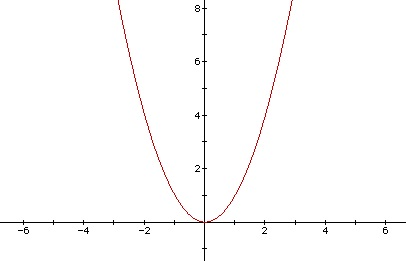
\includegraphics{Quadratic.jpg}

\newpage

\textbf{Graph of Cubic Function $\mathbf{y=x^3}$}

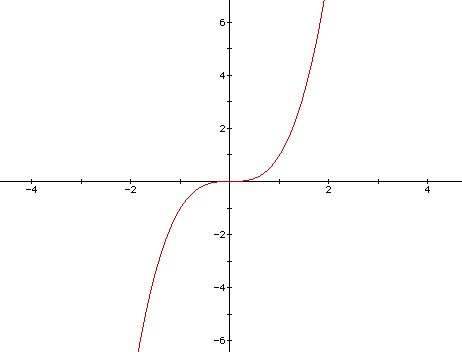
\includegraphics[scale = 0.9]{CubeFunction.jpg}

\textbf{Graph of Absolute Value $\mathbf{y=|x|}$}

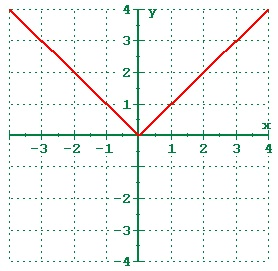
\includegraphics[scale = 0.9]{AbsoluteValue.jpg}

\textbf{Graph of Square Root $\mathbf{y=\sqrt{x} = x^{1/2}}$}

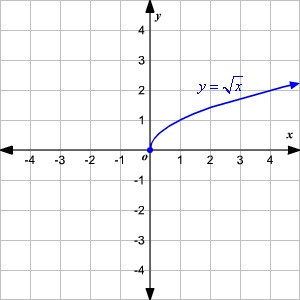
\includegraphics{SquareRoot.jpg}

\textbf{Graph of Cubic Root Function $\mathbf{y=\sqrt[3]{x} = x^{1/3}}$}

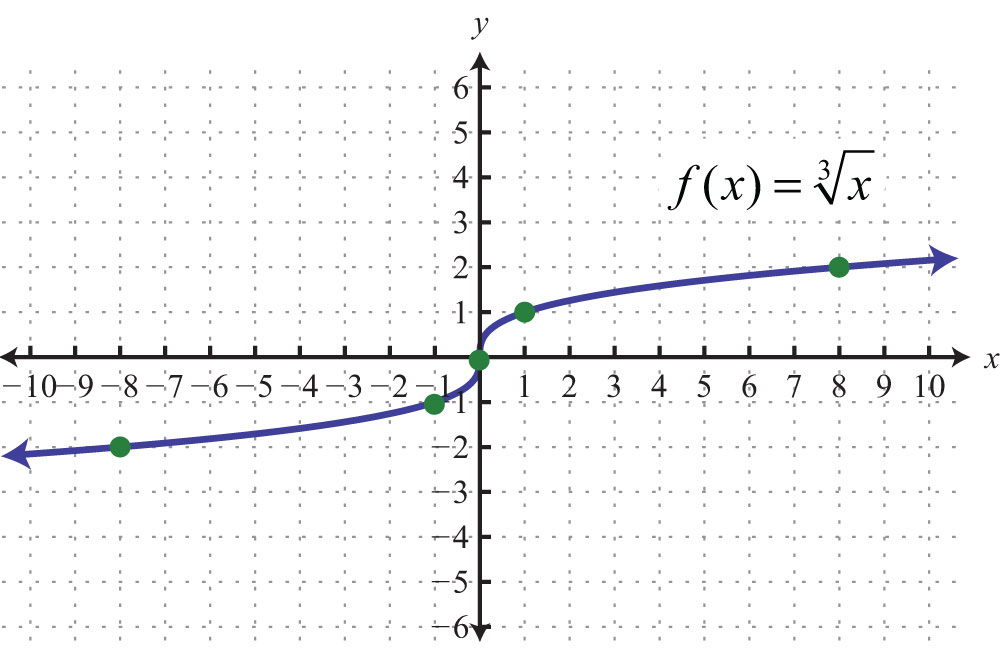
\includegraphics[scale = 0.3]{CubeRootFunction.jpg}

\textbf{Graph of the Reciprocal Function $\mathbf{y=\dfrac{1}{x}}$}

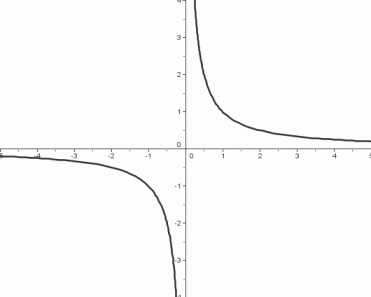
\includegraphics{RecipFunction.jpg}

\textbf{Increasing:} A function $f$ is \textit{increasing} if for any $x_{1}, x_{2}$ with $x_{1} < x_{2} \implies f(x_{1}) < f(x_{2})$

\textbf{Decreasing:} A function $f$ is \textit{decreasing} if for any $x_{1}, x_{2}$ with $x_{1} < x_{2} \implies f(x_{1}) > f(x_{2})$

\textbf{Constant:} A function $f$ is \textit{constant} if for any $x_{1}, x_{2}$ then $f(x_{1}) = f(x_{2})$

\textbf{Difference Quotient:}
\newline

\centerline{$\dfrac{f(x+h) - f(x)}{h}$}

\textbf{Internet Links:}

\href{https://www.youtube.com/watch?v=v5P4y0OkED4}{patrickJMT - Difference Quotient}

\newpage

\subsection{Transformations}

\textbf{Vertical Shifts:} Let $c>0$

\begin{enumerate}
\item $y=f(x) + c$ shifts $f(x)$ c units up
\item $y=f(x) - c$ shifts $f(x)$ c units down
\end{enumerate}

\textbf{Horizontal Shifts:} Let $c>0$

\begin{enumerate}
\item $y=f(x+c)$ shifts $f(x)$ c units left
\item $y=f(x-c)$ shifts $f(x)$ c units right
\end{enumerate}

\textbf{Reflections:} 

\begin{enumerate}
\item $y=-f(x)$ reflects $f(x)$ about the x-axis
\item $y=f(-x)$ reflects $f(x)$ about the y-axis
\end{enumerate}

\textbf{Vertical Stretch \& Shrink:} 
\newline

\centerline{Let $c>0$. We consider $y=cf(x)$}

\begin{enumerate}
\item $c>1 \hspace{.75cm} \to$ stretch $f(x)$ vertically by a factor of c
\item $0<c<1 \to$ shrink $f(x)$ vertically by a factor of c
\end{enumerate}
\vspace{.5cm}
\textbf{Horizontal Stretch \& Shrink:} 
\newline

\centerline{Let $c>0$. We consider $y=f(cx)$}

\begin{enumerate}
\item $c>1 \hspace{.75cm} \to$ shrink $f(x)$ horizontally by a factor of c
\item $0<c<1 \to$ stretch $f(x)$ horizontally by a factor of c
\end{enumerate}

\textbf{Order of Transformations:}

\begin{enumerate}

\item Horizontal Shift 
\item Stretch/Shrink 
\item Reflections
\item Vertical Shift

\end{enumerate}

\subsection{Combining Functions}

\textbf{Arithmetic Combinations of Functions:}

\begin{enumerate}
\item $(f+g)(x) = f(x) + g(x)$
\begin{myindentpar}{1cm}
\textbf{Example:} Let $f(x) = x^2+3x+7$ and $g(x) = -x+2$

Then $(f+g)(x) =  (x^2+3x+7) + (-x+2) = x^2+2x+9$

\end{myindentpar}
\item $(f-g)(x) = f(x) - g(x)$

\begin{myindentpar}{1cm}
\textbf{Example:} Let $f(x) = x^2+3x+7$ and $g(x) = -x+2$

Then $(f+g)(x) =  (x^2+3x+7) - (-x+2) = x^2+4x+5$

\end{myindentpar}

\item $(f \cdot g)(x) = f(x) \cdot g(x)$
\begin{myindentpar}{1cm}
\textbf{Example:} Let $f(x) = x^2$ and $g(x) = \dfrac{1}{x}$

Then $(f \cdot g)(x) =  (x^2) \cdot \Big(\dfrac{1}{x}\Big) = \dfrac{x^2}{x} = x$

\end{myindentpar}


\item $(\dfrac{f}{g})(x) = \dfrac{f(x)}{g(x)}$

\begin{myindentpar}{1cm}
\textbf{Example:} Let $f(x) = x^2+3x$ and $g(x) = \dfrac{1}{x^2}$

Then $(\dfrac{f}{g})(x) =  \dfrac{x^2+3x}{\dfrac{1}{x^2}} = x^2(x^2+3x) = x^4+3x^3$

\end{myindentpar}
\end{enumerate}

\textbf{Function Composition:} 

$(f \circ g)(x) = f \Big(g(x)\Big)$
\begin{myindentpar}{1cm}


\textbf{Example:} Let $f(x) = 3x^2-2$ and $g(x) = \dfrac{x+2}{x-1}$ 

Then $f \circ g = 3 \Big(\dfrac{x+2}{x-1} \Big)^2 -2$

\textbf{Note:} Be careful when finding the domain of a composition of functions. 
\end{myindentpar}
\begin{myindentpar}{2cm}
\textbf{Example:} Let $f(x) = \sqrt{x-12}$ and $g(x) = x^2-4$

Find 

a) $f \circ g$ 

b) $g \circ f$ 

and state the domain of each
\end{myindentpar}
\begin{myindentpar}{2.5cm}
\textbf{Answer:}
 \textbf{a)} $f \circ g = \sqrt{(x^2-4)-12}$

\hspace{3.3cm} $ = \sqrt{x^2-16}$

\textbf{Domain:} $x^2 - 16 \geq 0 \implies x\leq -4$ and $x \geq 4$

So the domain in interval notation is $(-\infty, -4] \cup [4, \infty)$

\textbf{Answer: b)} $g \circ f = \Big(\sqrt{x-12}\Big)^2 -4$

\hspace{3.3cm} $ = x-12 -4$

\hspace{3.3cm} $ = x-16$

\textbf{Domain:} $x - 12 \geq 0 \implies x \geq  12 \implies [12 , \infty)$
\end{myindentpar}

\subsection{One-to-One Functions and Inverse Functions}


\textbf{One-to-One Algebraic Test:} Set $f(x_{1}) = f(x_{2})$ and show $x_{1} = x_{2}$ ONLY

\begin{myindentpar}{1cm}
\textbf{Horizontal Line Test:} - a nice, easy, graphical test to determine if a function is one-to-one. It says that a function is \textbf{one-to-one} if every horizontal line intersects a graph \textbf{at most once}

\newpage

\textbf{Function That Passes the Horizontal Line Test:}

\centerline{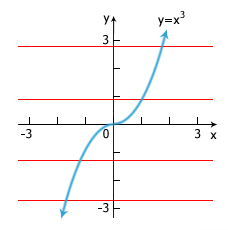
\includegraphics{PassHLT.jpg}}

\textbf{Function That Fails Horizontal Line Test:}

\centerline{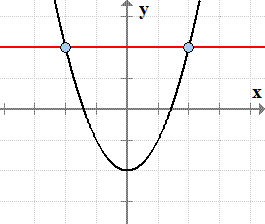
\includegraphics{FailHLT.png}}

\end{myindentpar}

\textbf{Inverse Function:} - if a function $f$ is one-to-one then the \textbf{inverse function} denoted by $f^{-1}(x)$ is the function that "undoes" the original function $f$ so that $f^{-1}\Big(f(x)\Big) = x$ 

\begin{itemize}
\item The domain of $f^{-1}$ is the range of $f$
\item The range of $f^{-1}$ is the domain of $f$
\item Graphically, the inverse function, $f^{-1}(x)$, is the graph of the original function, $f(x)$,  reflected about the line $y=x$
\end{itemize}

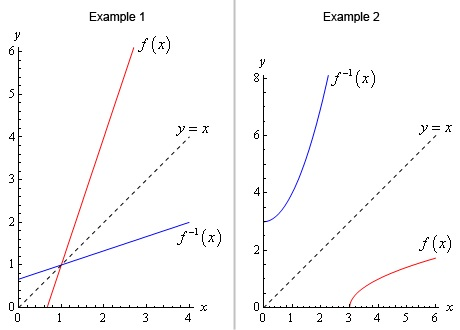
\includegraphics{InverseGraph.jpg}

\textbf{Note:} Notice how in Example 2 that the range of $f^{-1}(x)$ is the domain of $f(x)$

\textbf{Finding the Inverse Function:}

\begin{enumerate}
\item Set $y = f(x)$
\item Swap $x$ and $y$
\item Solve for $y$ in terms of $x$
\item Done!
\end{enumerate}

\section{Chapter 1: Polynomials and Rational Functions}

\subsection{Quadratic Functions}

\textbf{Standard Form of a Quadratic Function:}
\newline

\centerline{$f(x) = a(x-h)^{2} + k$}

\hspace{6.5cm} Vertex: $(h,k)$

\hspace{6.5cm} $a > 0 \to$ Upward Pointing

\hspace{6.5cm} $a < 0 \to$ Downward Pointing

\textbf{Vertex of a Parabola:}
\newline

\centerline{$\Big(-\dfrac{b}{2a}, f(-\dfrac{b}{2a}) \Big)$}

\newpage

\subsection{Polynomial Functions of Higher Degree}

\textbf{Multiplicity of a Zero:}
\newline

\begin{itemize}
\item If $(x-a)^{n}$ is a factor of a polynomial, then $a$ is called a zero of multiplicity $n$
\item $n \text{ even} \to $ function does not change sign
\item $n \text{ odd} \to $ function changes sign 
\end{itemize}

\subsection{Dividing Polynomials}

There are 2 methods used to divide polynomials:

\begin{enumerate}
\item Long Division
\item Synthetic Division
\end{enumerate}

Long division can ALWAYS be used to divide polynomials. 

Synthetic division can ONLY be used when \textbf{dividing by a linear factor}

I will list some internet links because they can do a much better job explaining both of these methods than I can in here.

\textbf{Internet Links:}

\begin{itemize}
\item \href{https://www.youtube.com/watch?v=Ih1wb6AxhMI}{mathbff - Long Division} 

\item \href{https://www.youtube.com/watch?v=l6_ghhd7kwQ}{patrickJMT - Long Division}

\item \href{https://www.youtube.com/watch?v=FXgV9ySNusc}{Khan Academy - Long Division}

\item \href{https://www.youtube.com/watch?v=lLgRS0mUZLw}{mathbff - Synthetic Division} 

\item \href{https://www.youtube.com/watch?v=bZoMz1Cy1T4}{patrickJMT - Synthetic Division}

\item \href{https://www.youtube.com/watch?v=1byR9UEQJN0}{Khan Academy - Synthetic Division}

\end{itemize}

\subsection{The Real Zeros of a Polynomial Function}

\textbf{Remainder Theorem:} 
\newline

\centerline{If a polynomial $P(x)$ is divided by $x-a$, then the remainder is $r = P(a)$}

\textbf{Factor Theorem:} 
\newline

\centerline{If $P(a) = 0$, then $x - a$ is a factor of $P(x)$. Conversely, if $x-a$ is a factor of $P(x)$, then $P(a) = 0$ }

\textbf{Number of Real Zeros:} 
\newline

\centerline{A polynomial cannot have more \textbf{real zeros} than its degree}

\textbf{Rational Zero Theorem:} If a polynomial function has \textbf{integer coefficients}, then every \textbf{rational zero} of $P(x)$ has the form:
\newline

\centerline{Rational Zero = $\pm \dfrac{\text{positive integer factors of constant term}}{\text{positive integer factors of leading coefficient}}$}

\textbf{Descartes Rule of Signs:} For a polynomial with real coefficients the following two things are true:
\newline

\begin{enumerate}
\item The number of \textbf{positive real zeros} of the polynomial is either equal to the number of changes of sign of $P(x)$ or less than that number by an even integer
\item The number of \textbf{negative real zeros} of the polynomial is either equal to the number of changes of sign of $P(-x)$ or less than that number by an even integer
\end{enumerate}

\subsection{Complex Zeros: The Fundamental Theorem of Algebra}

\centerline{\textbf{NOT COVERED ON MIDTERM}}

\subsection{Rational Functions}

\textbf{Vertical Asymptotes:} 

The line $x = a$ is a \textbf{vertical asymptote} for the graph of a function if $f(x)$ either increases or decreases without bound as $x$ approaches from either the right or left.  

\centerline{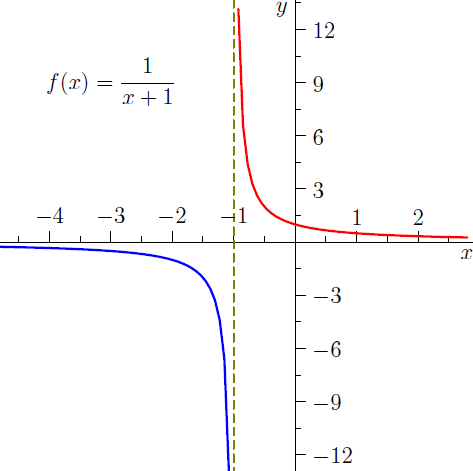
\includegraphics[scale = 0.5]{VerticalAsymptote.png}}

\textbf{Finding Vertical Asymptotes:} Set the denominator equal to $0$

\textbf{Horizontal Asymptotes:} 

The line $y = a$ is a \textbf{horizontal asymptote} for the graph of a function if $f(x)$ approaches $a$ as $x$ increases or decreases without bound

\centerline{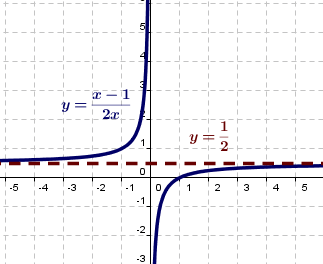
\includegraphics[scale = 0.7]{HorizontalAsymptote.png}}

\textbf{Finding Horizontall Asymptotes:} Compare of the degree of the numerator and the denominator of a rational function. 

\begin{enumerate}
\item When the degree of the numerator is less than the degree of the denominator, then $y = 0$ is the horizontal asymptote
\item When the degree of the numerator is the same as the degree of the denominator, then the horizontal asymptote is the ratio of the leading coefficients in the numerator and denominator
\item When the degree of the numerator is greater than the degree of the denominator, then there is no horizontal asymptote
\end{enumerate}

\textbf{Slant Asymptotes:} 

If $f(x) =\dfrac{n(x)}{d(x)}$ where $n(x)$ and $d(x)$ are polynomials and the degree of $n(x)$ is one more than the degree of $d(x)$ the slant asymptote is given by dividing $n(x)$ by $d(x)$. The result after doing the division allows us to write $f(x)$ in the following way:
\newline

\centerline{$f(x) = mx + b + \dfrac{r(x)}{d(x)}$}

Then $y = mx+b$ is the slant asymptote for the graph of $f$

\centerline{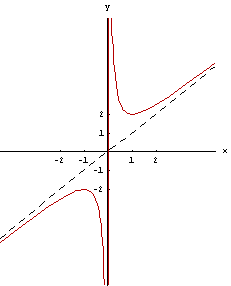
\includegraphics{SlantAsymptote.png}}
































\end{document}